\section{Figures and Tables}

There is a limit of 6 tables and figures in the paper.

\begin{table}[H]
\begin{center}
\begin{tabular}{ |l|c|c|c|c| } 
 \hline
 Drug & Trastuzumab & Pembrolizumab & Atezolizumab & Bevacizumab \\ 
 Target Type & Membrane-Bound & Membrane-Bound & Membrane-Bound & Soluble \\
 Target & HER2 & PD-1 & PD-L1 & VEGF \\ 
 Baseline Target (nM) & X & Y & Z & A \\ 
 Other info?\\
 \hline
\end{tabular}
\end{center}
\caption{Summary of drugs in this analysis.  Listing all the parameters is probably a bit nuts.  I'd rather refer the reader to teh spreadsheet and also in the appendix or supplementary material we can give more information.}
\end{table}

\begin{figure}[H]
\centering
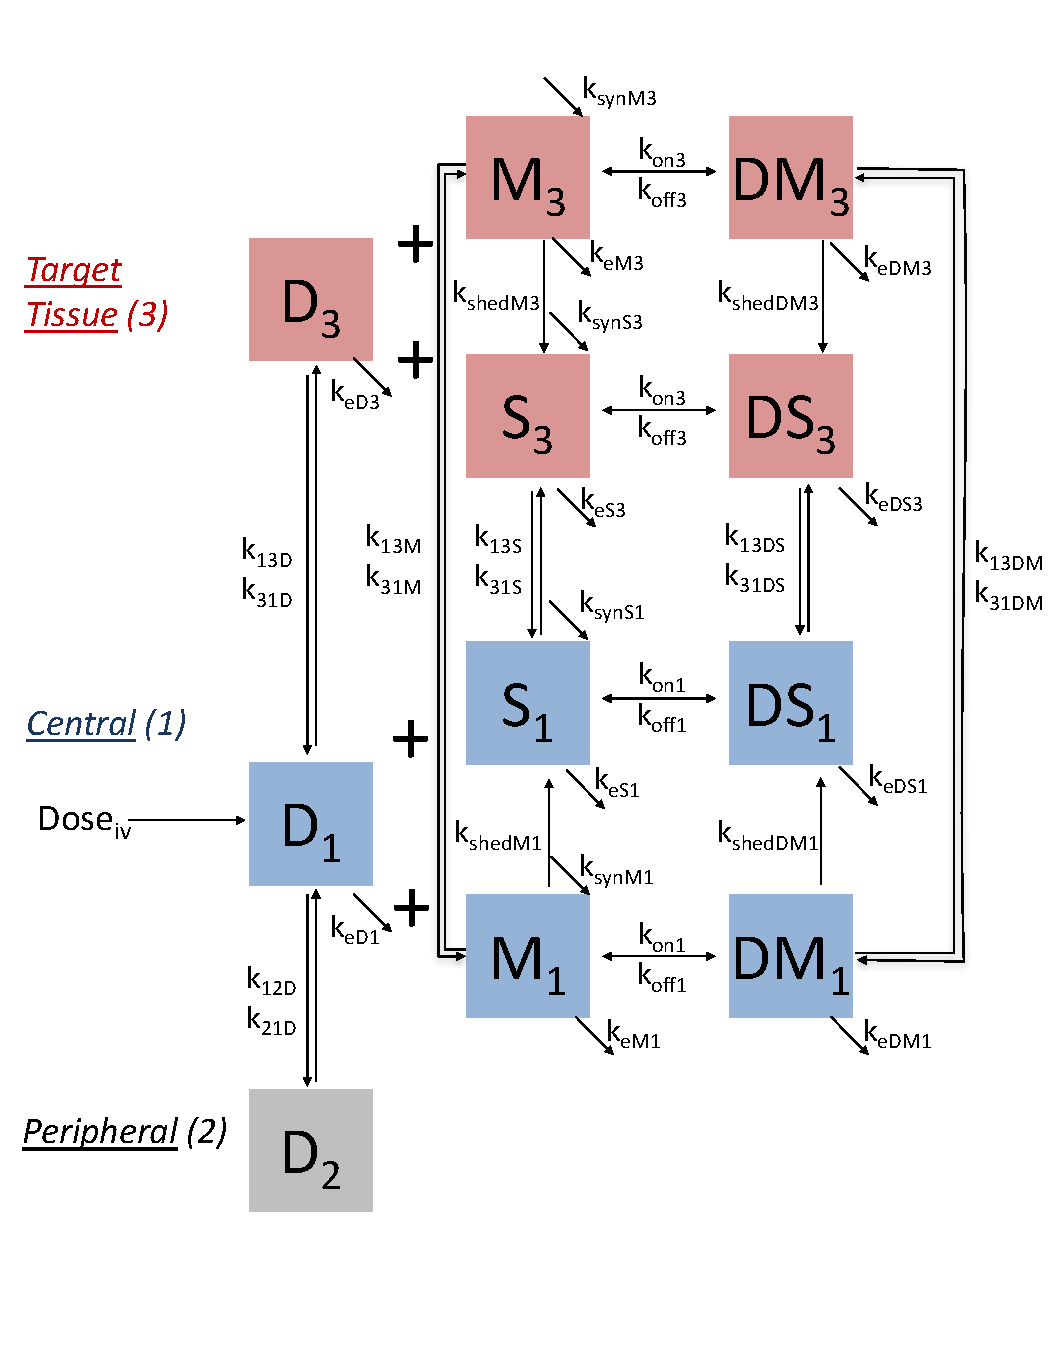
\includegraphics[width=\textwidth]{figures/ivsc_3cmtct_sm_full.pdf}
\caption{The extended target mediated drug disposition model.  Vertical arrows represent distribution, horrizontal arrows represent dosing and binding, and diagonal arrows represent synthesis and elimination. 
\label{fig:model}}.
\end{figure}

\begin{figure}[H]
\centering
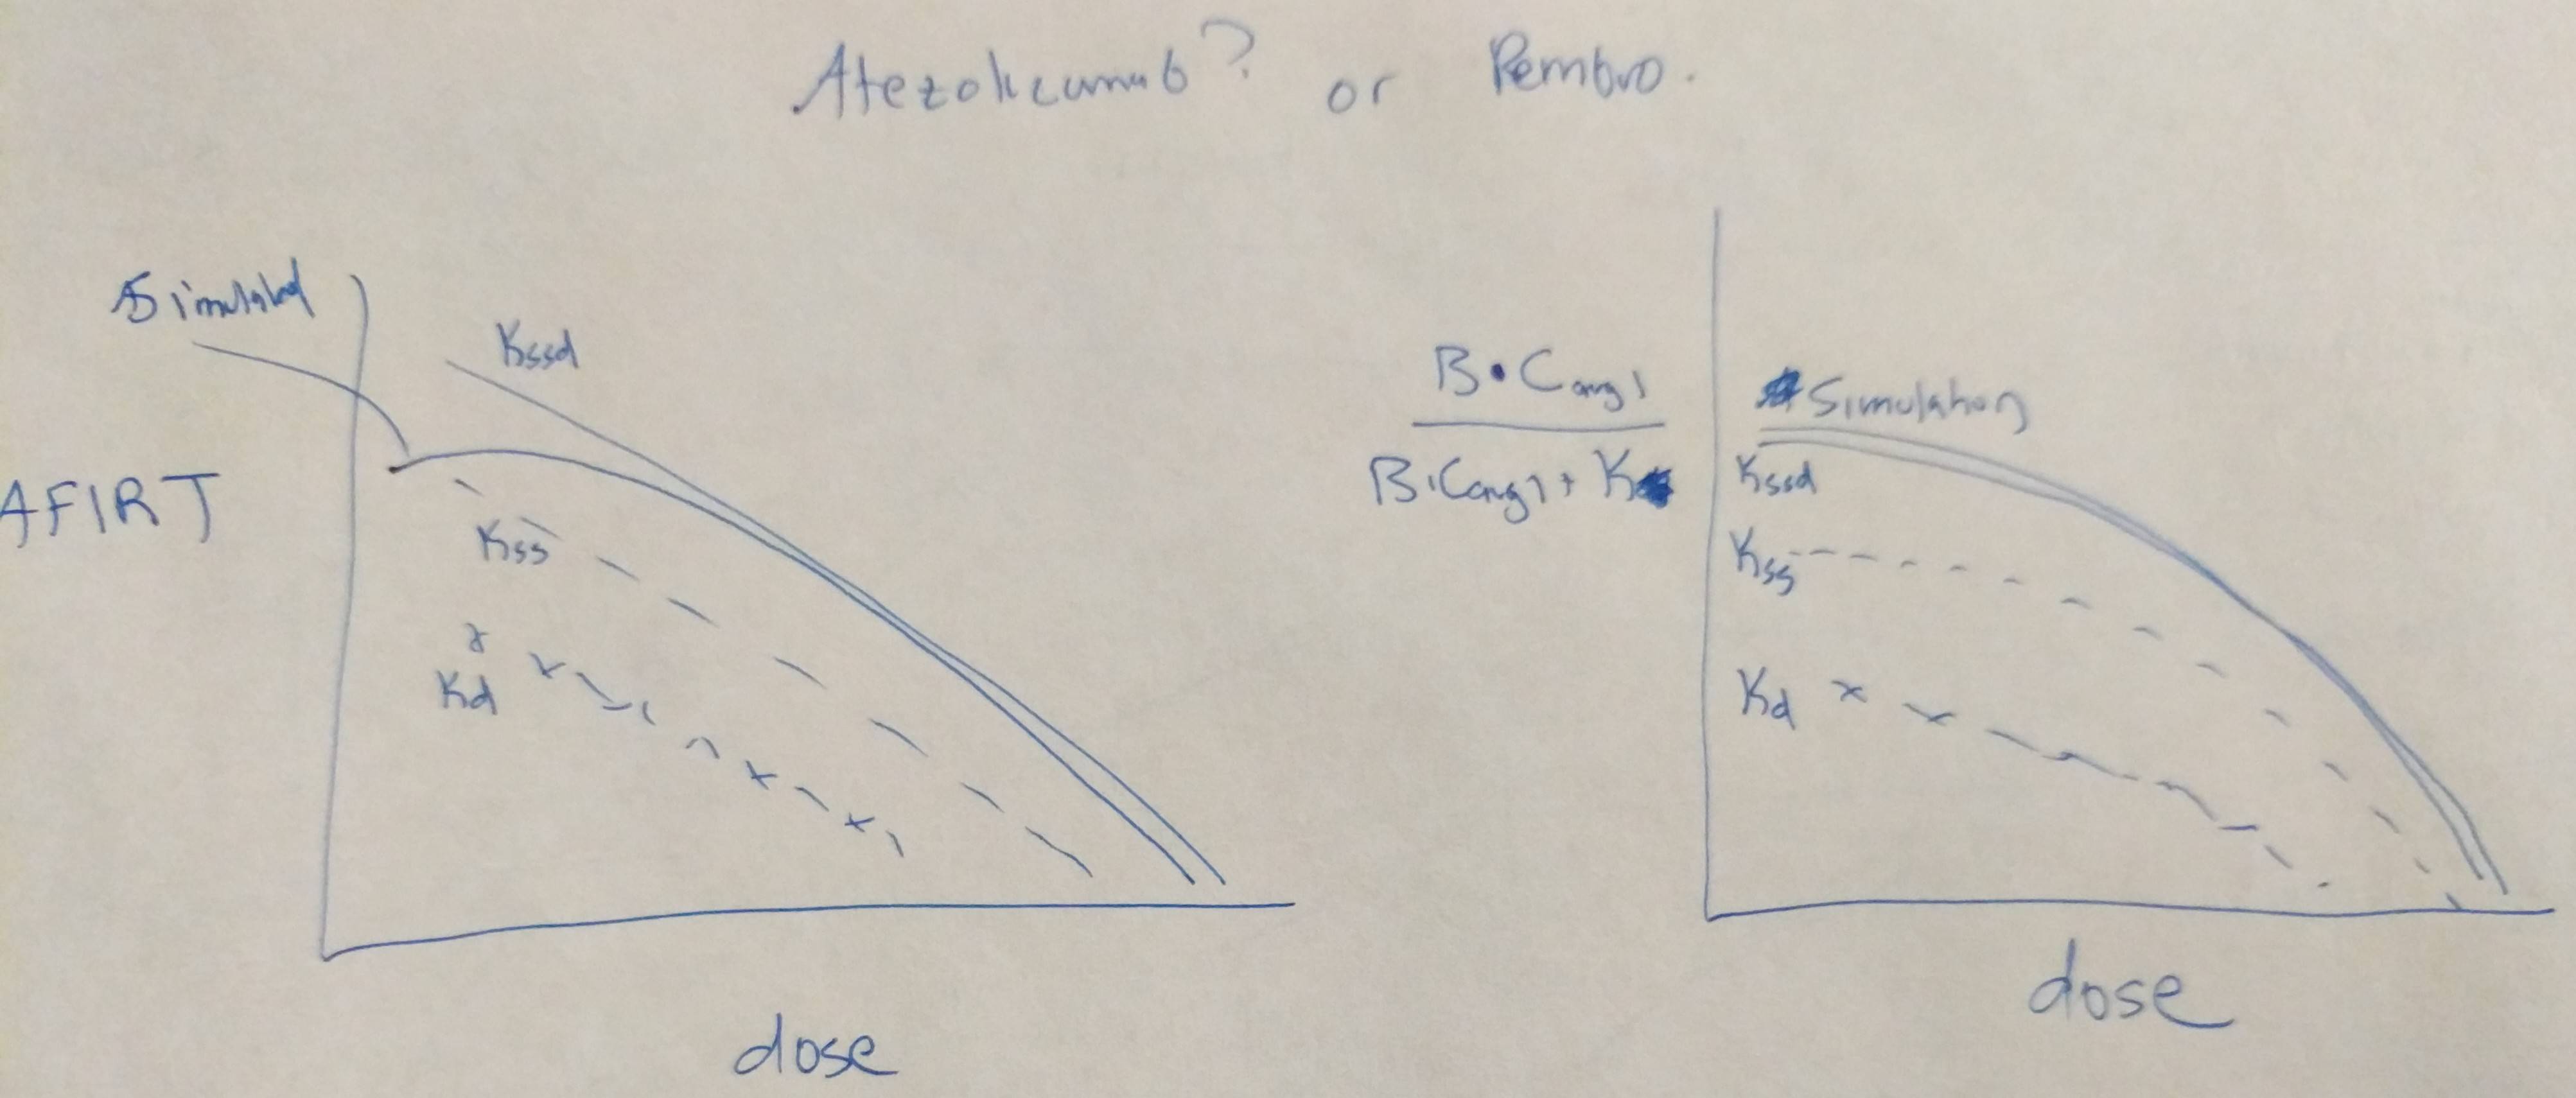
\includegraphics[width=\textwidth]{figures/Kssd_Kss_Kd.jpg}
\caption{Here we show Kd, Kss, Kssd and that Kssd is superior for describing the data.  Might want to show for all four drugs and that Kssd will be superior for atezo and pembro, though maybe all will be terrible for herceptin.
\label{fig:Kssd}}.
\end{figure}

\begin{figure}[H]
\centering
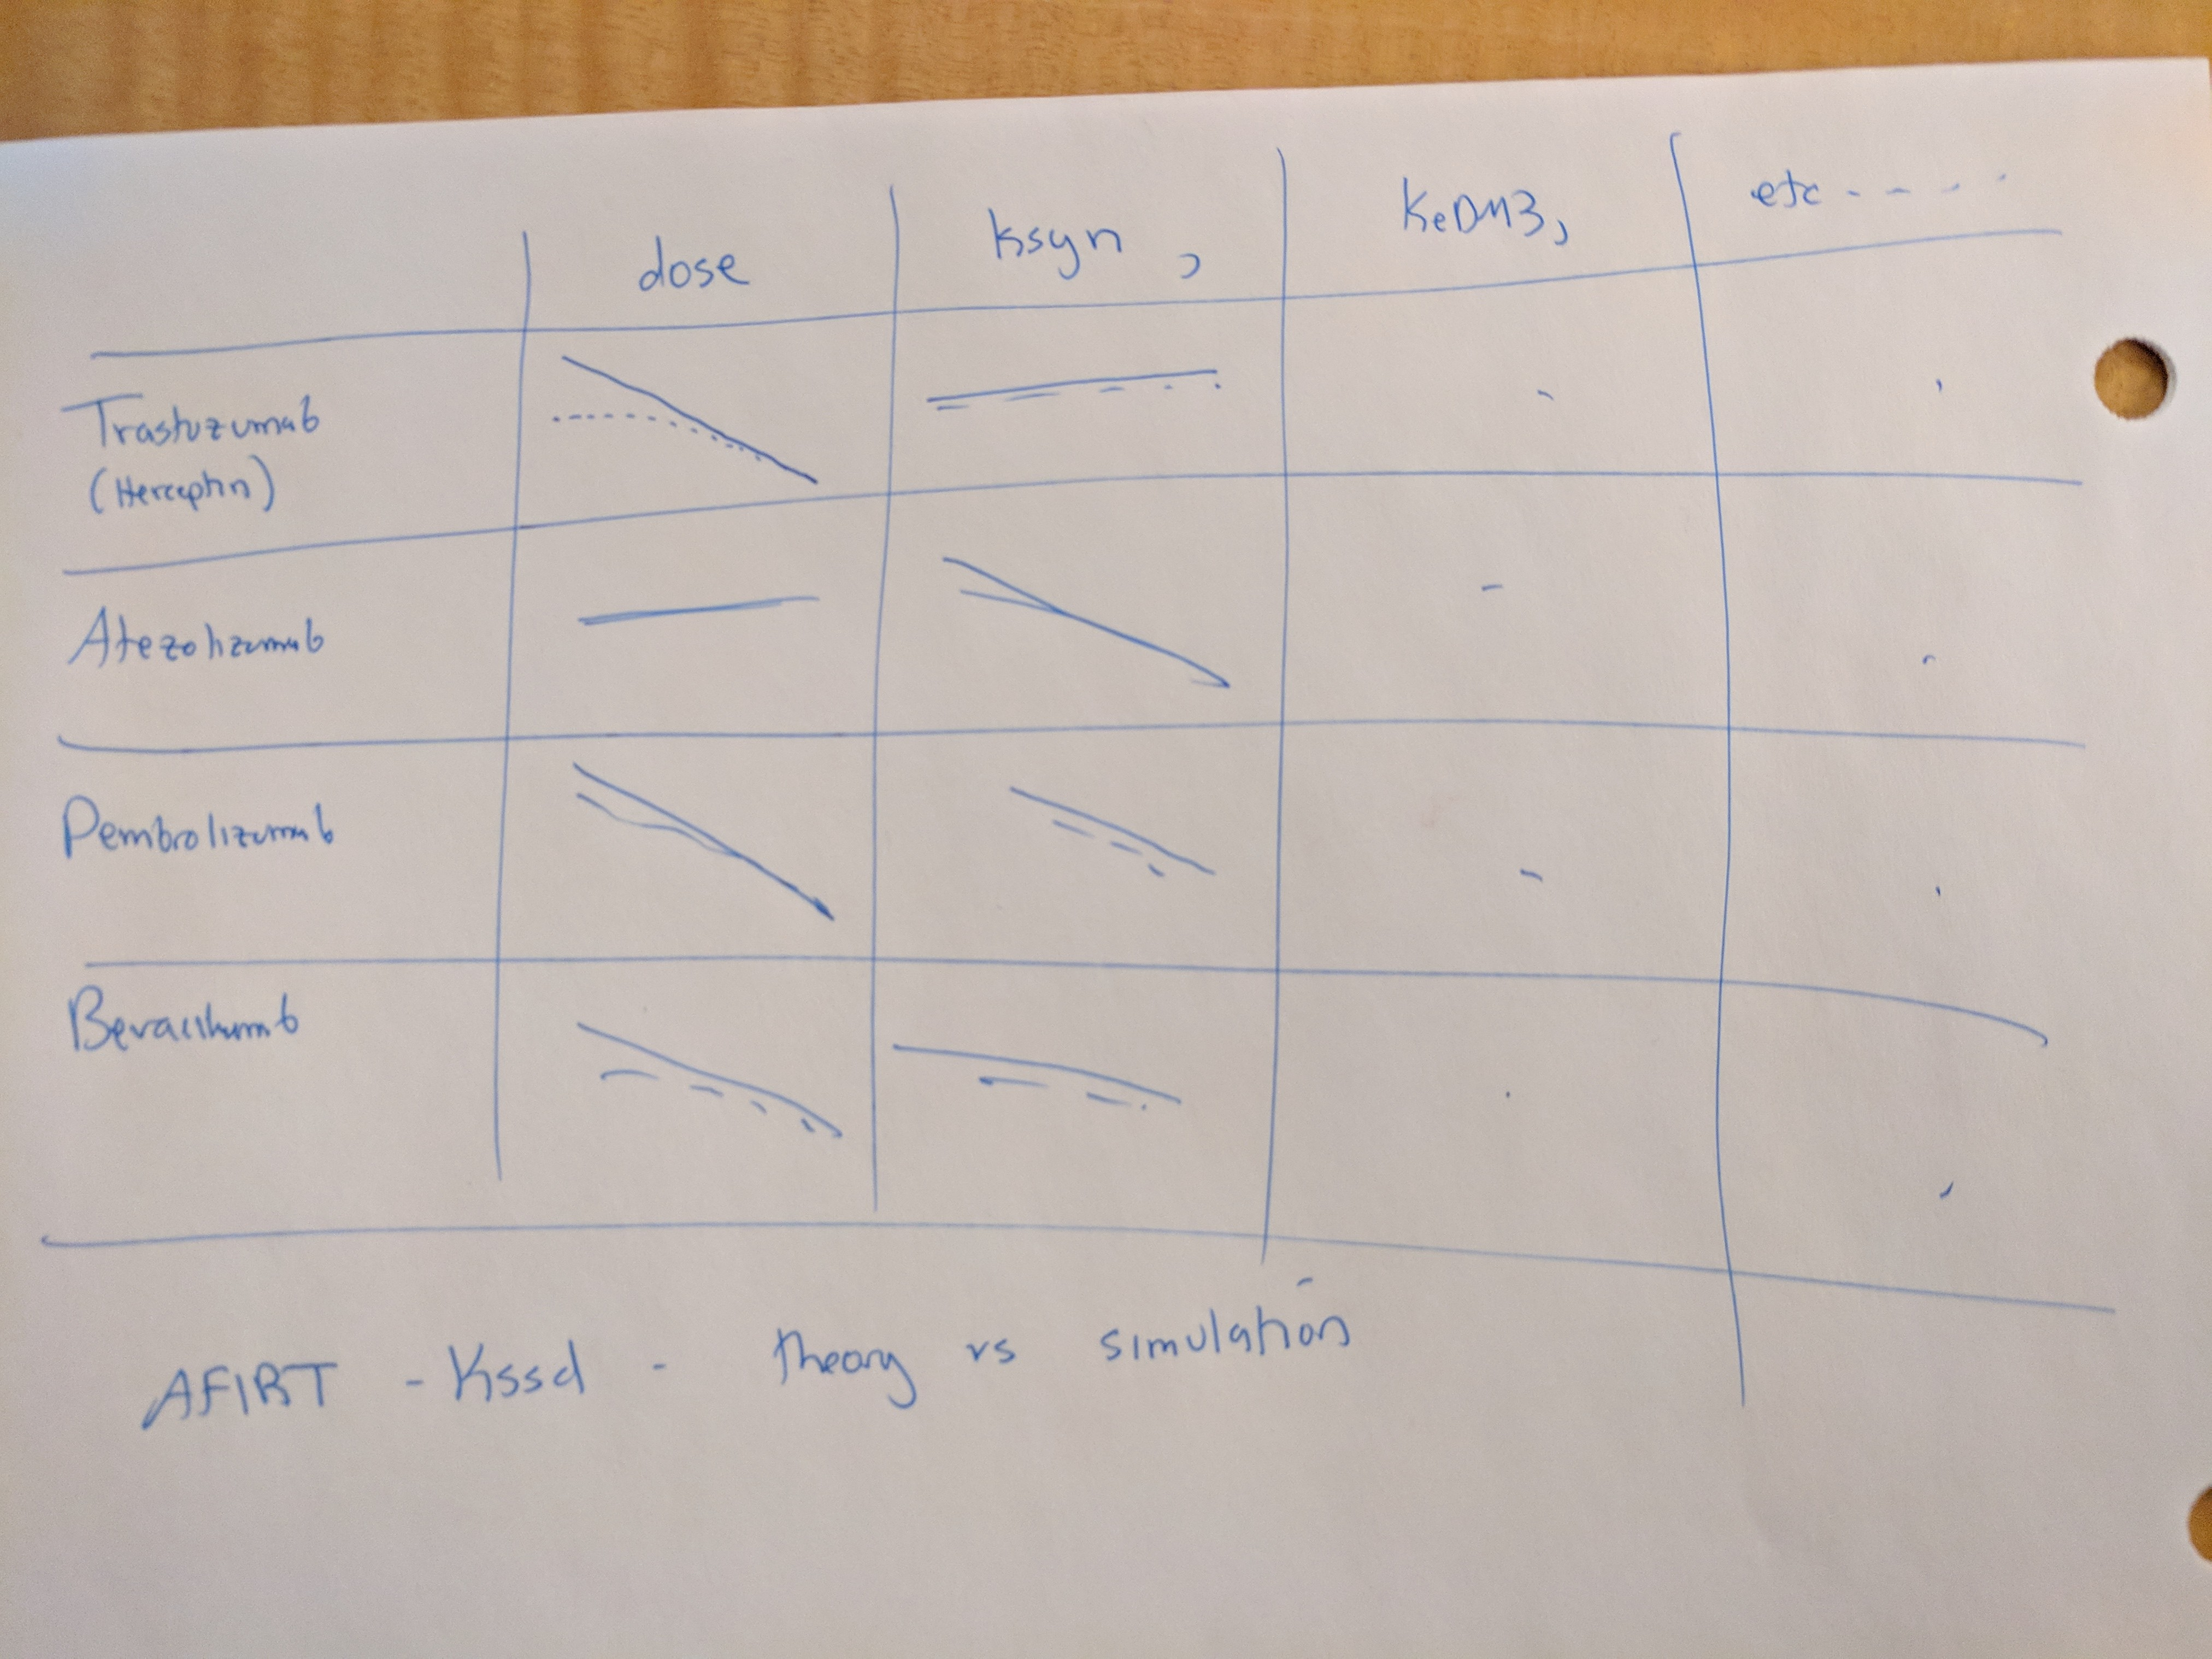
\includegraphics[width=\textwidth]{figures/SensitivityAnalysis.jpg}
\caption{Sensitivity analysis that Sameed is currently working on (building off Hongshan's initial code).  This will show the accuracy of the AFIRT (or lack there of) over a wide range of scenarios)
\label{fig:sensitivity}}.
\end{figure}

\begin{figure}[H]
\centering
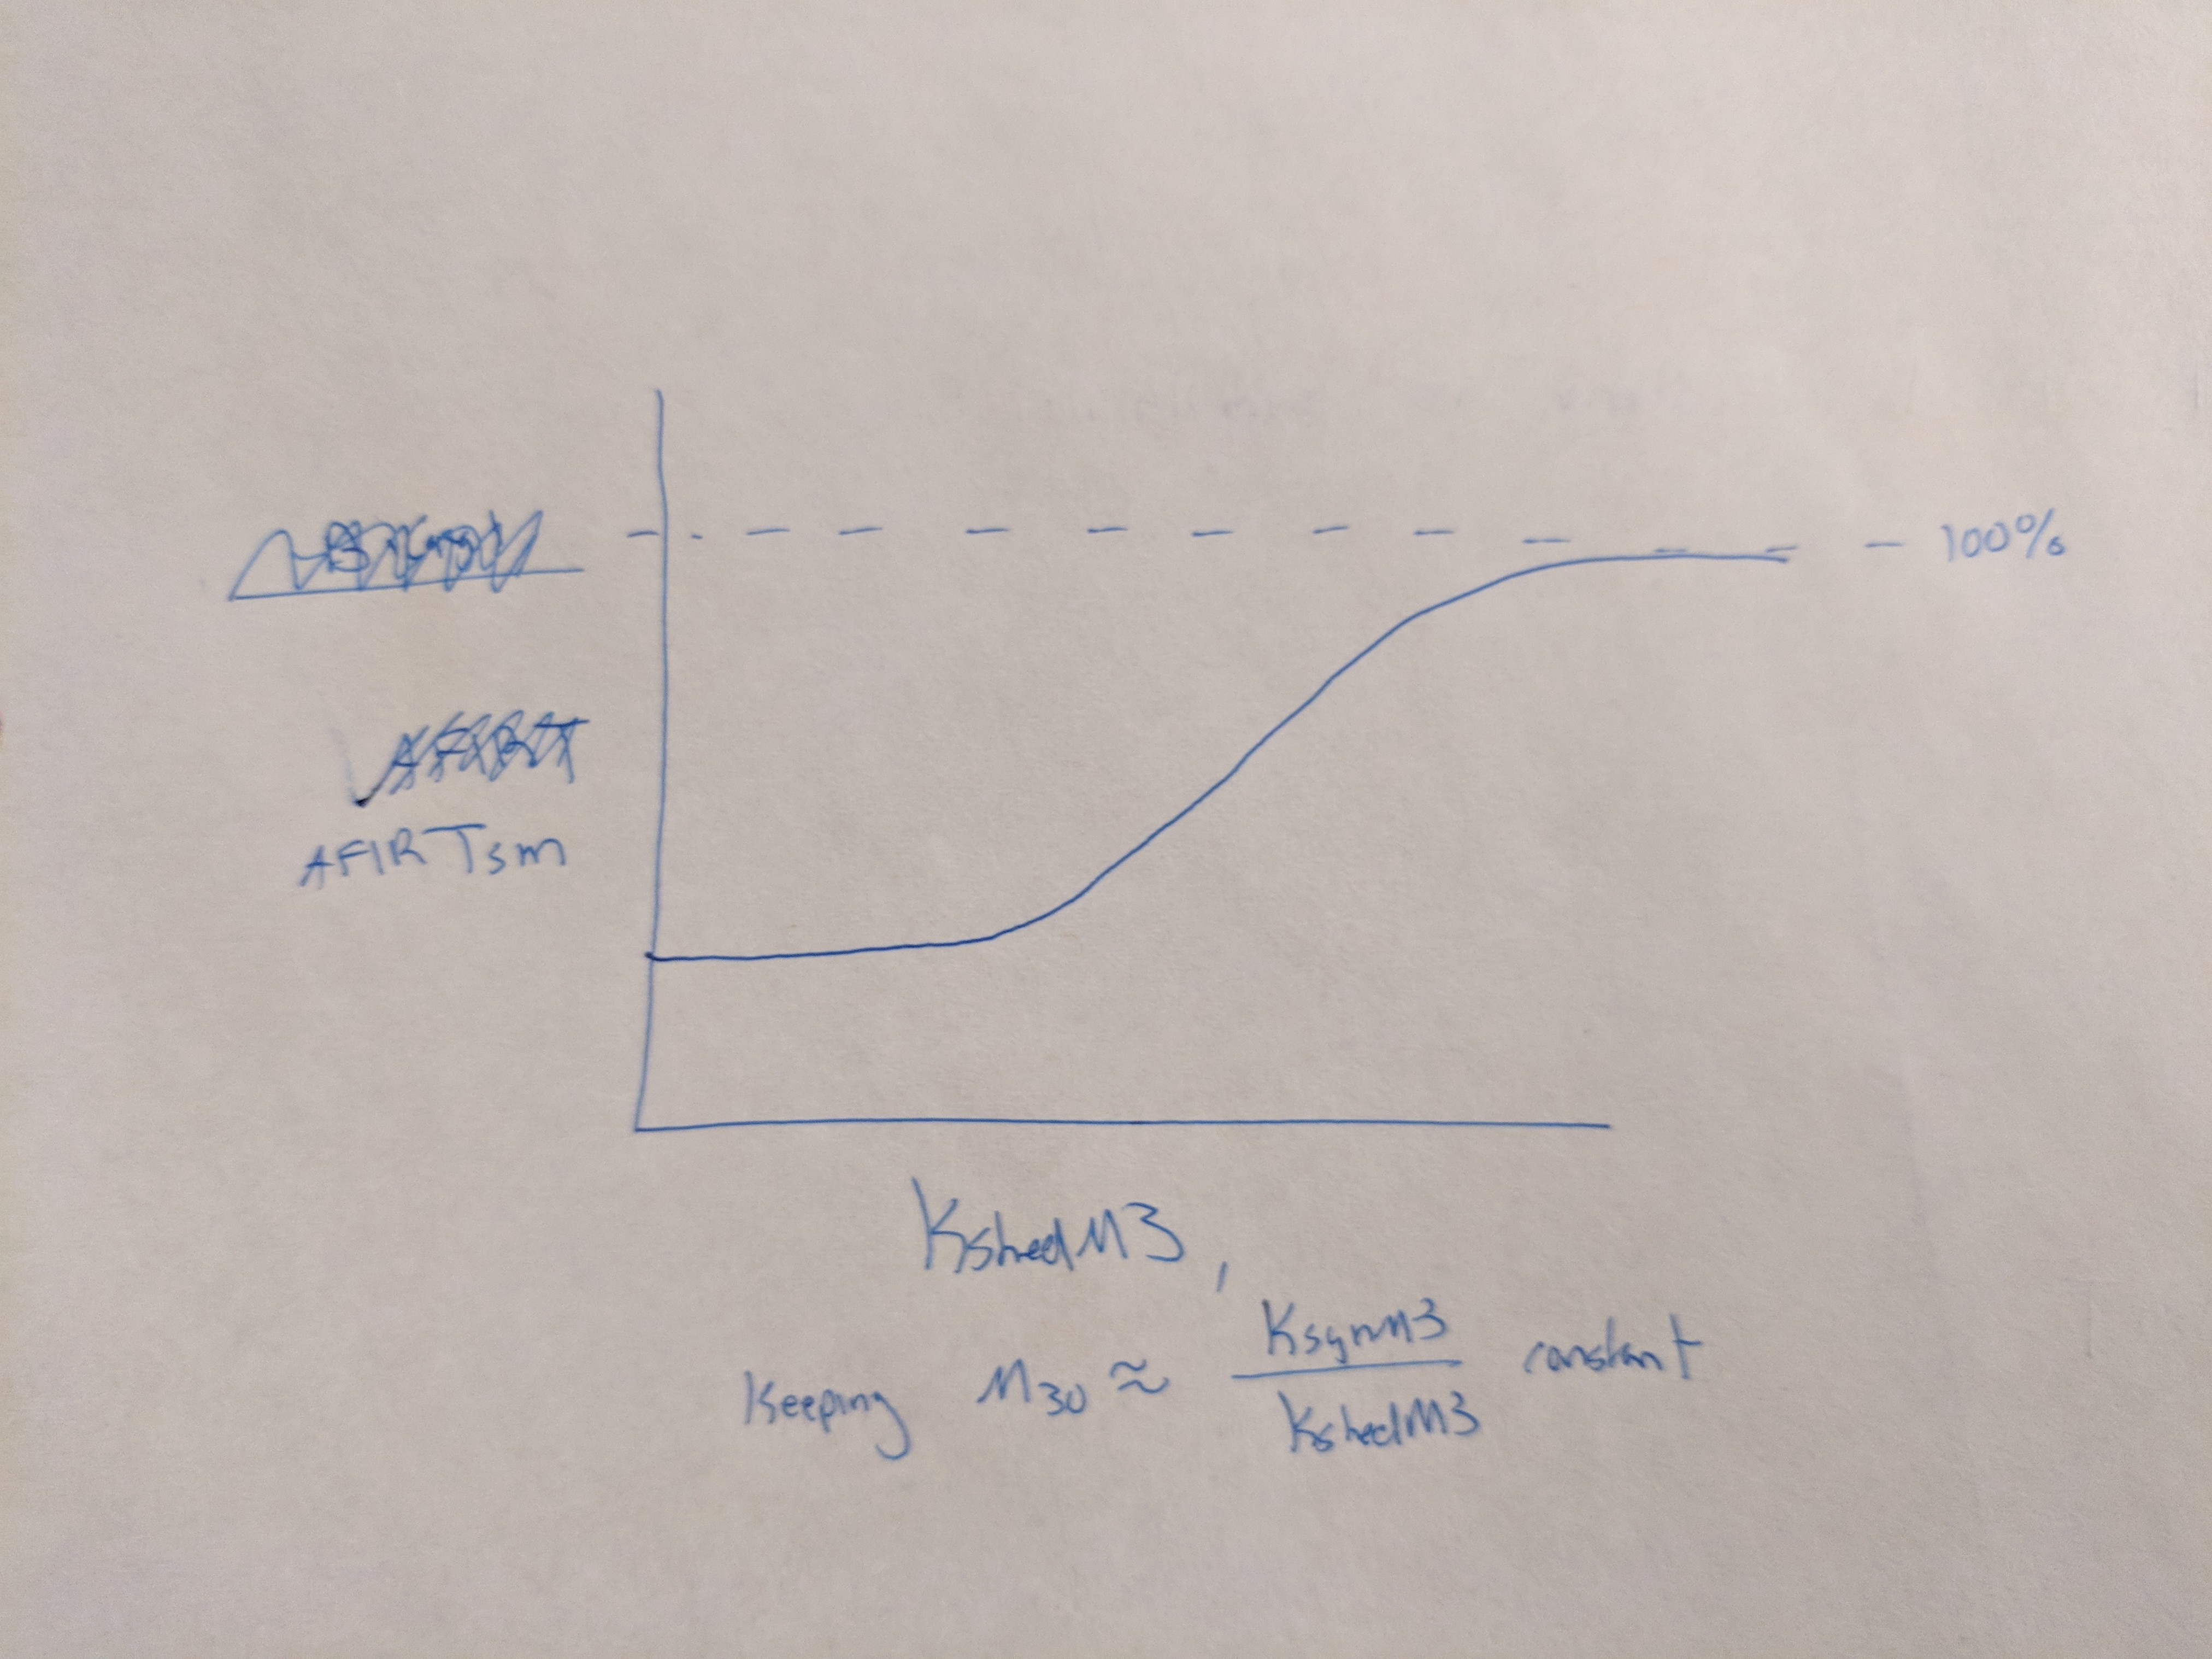
\includegraphics[width=\textwidth]{figures/FastShedding.jpg}
\caption{This will show that if the shedding is super fast, inhibiting the target is impossible.  This can also I think readily be seen from the Kssd equation. 
\label{fig:shedding}}.
\end{figure}

\begin{figure}[H]
\centering
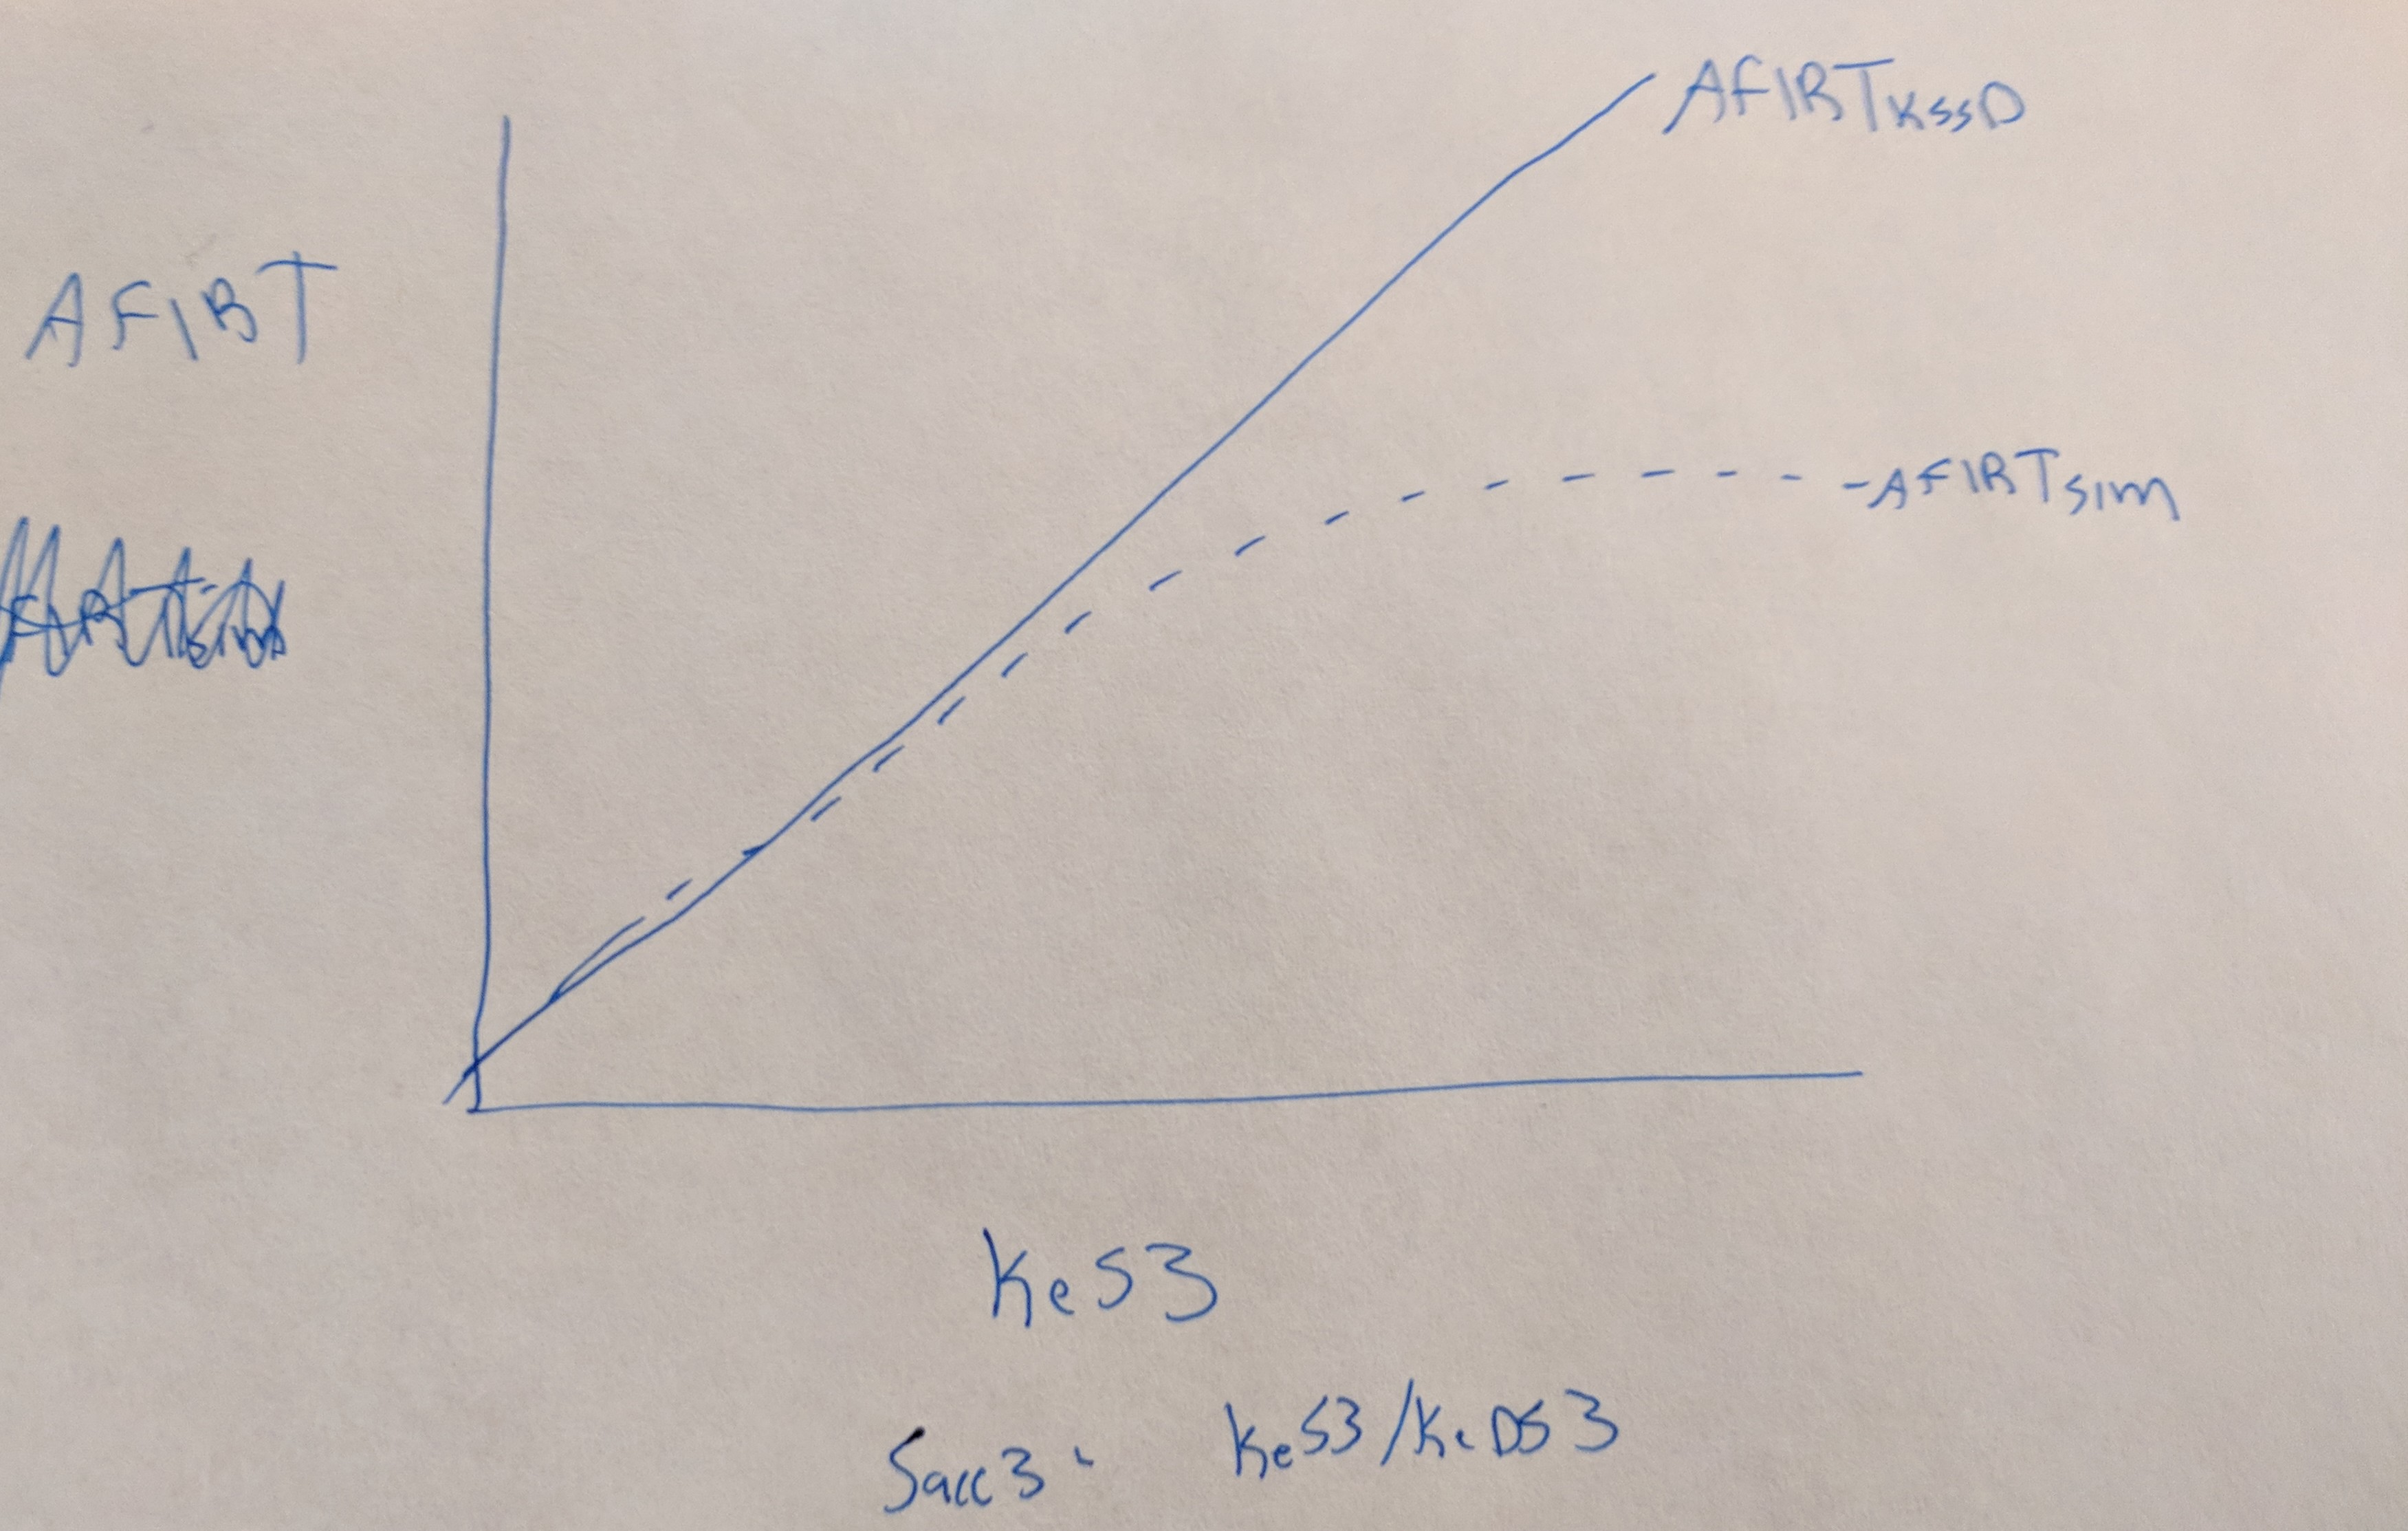
\includegraphics[width=\textwidth]{figures/SolubleAccumulation.jpg}
\caption{This will show that understanding the accumulation of the target in the tissue is critical.  But this is often not measured.  
\label{fig:accumulation}}.
\end{figure}

WE MIGHT WANT ONE MORE FIGURE LOOKING AT THE ACCURACY OF $\Kssd$ AS THE DISTRIBUTION BECOMES SLOW OR FAST.